
L'interface de la station de base est plut�t simple comme le d�montre la figure suivante \ref{f:InterfaceImage}. Elle a comme particularit� d'afficher une image virtuelle la plus semblable possible � l'image per�ue par la CameraMonde.
\medbreak

\begin{figure}[htp]
   \centering
   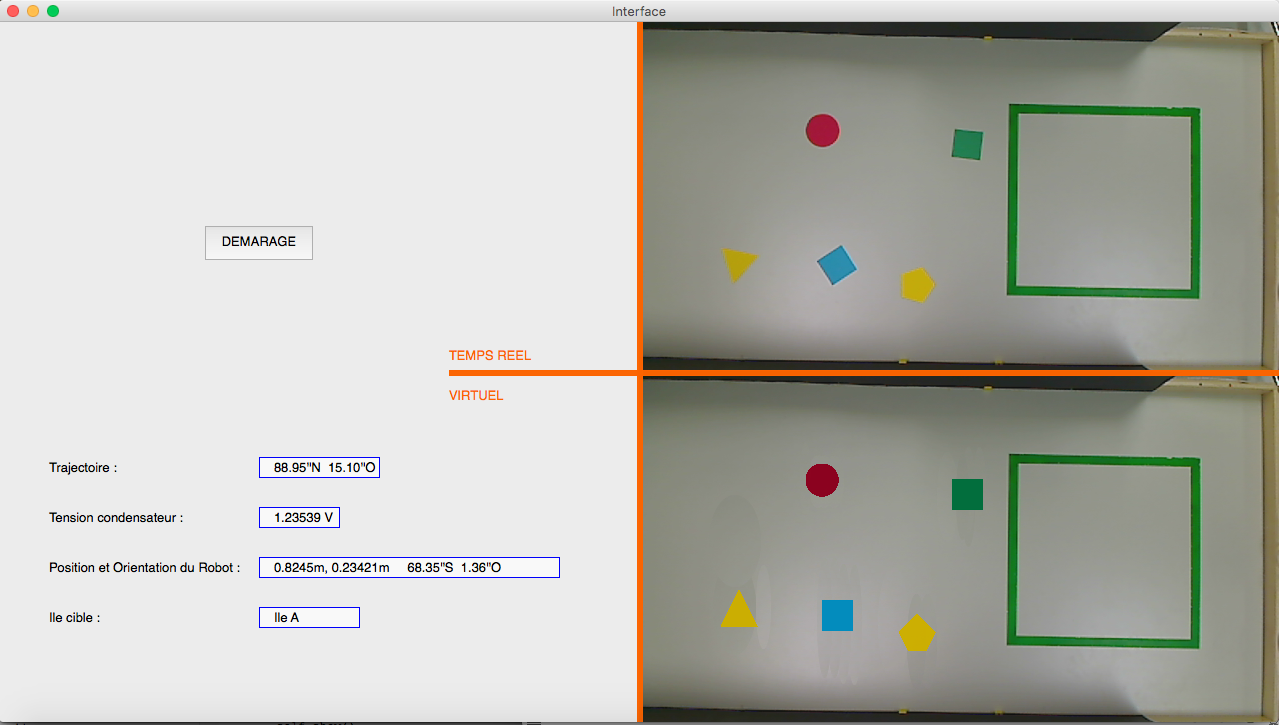
\includegraphics[width=1\textwidth]{fig/interface_Image.png}
   \caption{Interface de la station de base}
   \label{f:InterfaceImage}
\end{figure}

\medbreak
La section gauche de l'interface nous donne des informations sur le d�marage de la chasse au tr�sor en g�n�ral. Elle affiche �galement des informations pertinentes sur le robot comme l'�le cible, l'orientation, la position et la direction du robot ainsi que la tension dans le condensateur.
\medbreak
Pour l'instant, l'interface n'est pas connect�e au syst�me, mais elle est plut�t pr�t � recevoir des commandes tel que la position, la forme et la couleur d'un objet pour la reproduire de fa�on plut�t similaire dans notre image virtuelle comme le d�montre la partie inf�rieure droite de l'interface.
\medbreak
Le point fort de l'interface est l'id�e d'utiliser une photo de la Cam�raMonde avant que les objets soient ins�r�s ou que le robot soit ins�r� pour ensuite ajouter des objets virtuellement. Cel� nous aidera beaucoup plus � savoir si notre syst�me saisi bien les formes, les emplacements et les couleurs de toutes sortes � l'oeil nu. On devrait obtenir une image semblable la figure \ref{f:InterfaceImage} pr�c�dente dans la section virtuelle en bas � droite. On constate sur la figure que l'image en temps r�el est tr�s semblable � sa reproduction.

La forme et la couleur sur le dessus du robot pour pouvoir bien d�terminer l'orientation et la position du robot n'ont toujours pas �t� d�termin�es. Par contre, lorsqu'elle sera d�termin�. Il sera n�cessaire de l'afficher avec une bonne orientation (contrairement aux objets sur la map, bien qu'il serait int�ressant �galement de reproduire des objets dans leurs bons angles.)
\medbreak

 Il sera int�ressant aussi potentiellement d'afficher la trajectoire du robot sur la map virtuelle. Pour voir s'il suit bien sa trajectoire pour des tests. Et �galement un bouton stop pour arr�ter les op�rations du robot. Ceci nous permettrait de perdre moins de temps lorsqu'on voit qu'il y a quelque chose qui ne marche pas dans les commandes du robot et de la station de base.
